Our process of discovery of the constancy of $r/R$ started with picking a particular $a/b$ and plotting $R$, $r_9$, and $r$ vs. the $t$ parameter in $P_1(t)$; see Figure~\ref{fig:radii-grid2} (top). This confirmed the well-known relation $R/r_9=2$, valid for any triangle \cite{coxeter67}. It also suggested  that $R$ might be proportional to $r$, which is not true for any triangle family.

To investigate this potential relationship, we produced a scatter plot of orbit triangles for a discrete set of $a/b$ in $(r,R)$-space. One notices that triangles corresponding to individual $a/b$ fall on straight-line segments, and that all segments pass through the origin, suggesting that $r/R$ is a constant; see Figure~\ref{fig:radii-grid2} (bottom). One also notices each segment has endpoints $(R_\text{min},r_\text{min})$ and $(R_\text{max},r_\text{max})$. These are produced at isosceles orbit configurations (see Figure~\ref{fig:rR-min-max}) and are of the form

\begin{align}
r_{\mathrm{min}}=&  \frac{b^2(\delta - b^2)}{c^2 a},\;\;\;R_{\mathrm{min}}= \frac{a^2+\delta}{2a} \nonumber \\
r_{\mathrm{max}}=&  \frac{a^2(a^2 - \delta)}{c^2 b},\;\;\;R_{\mathrm{max}}= \frac{b^2+\delta}{2b}
\label{eqn:rmin-rmax}
\end{align}

\begin{figure}[H]
    \centering
    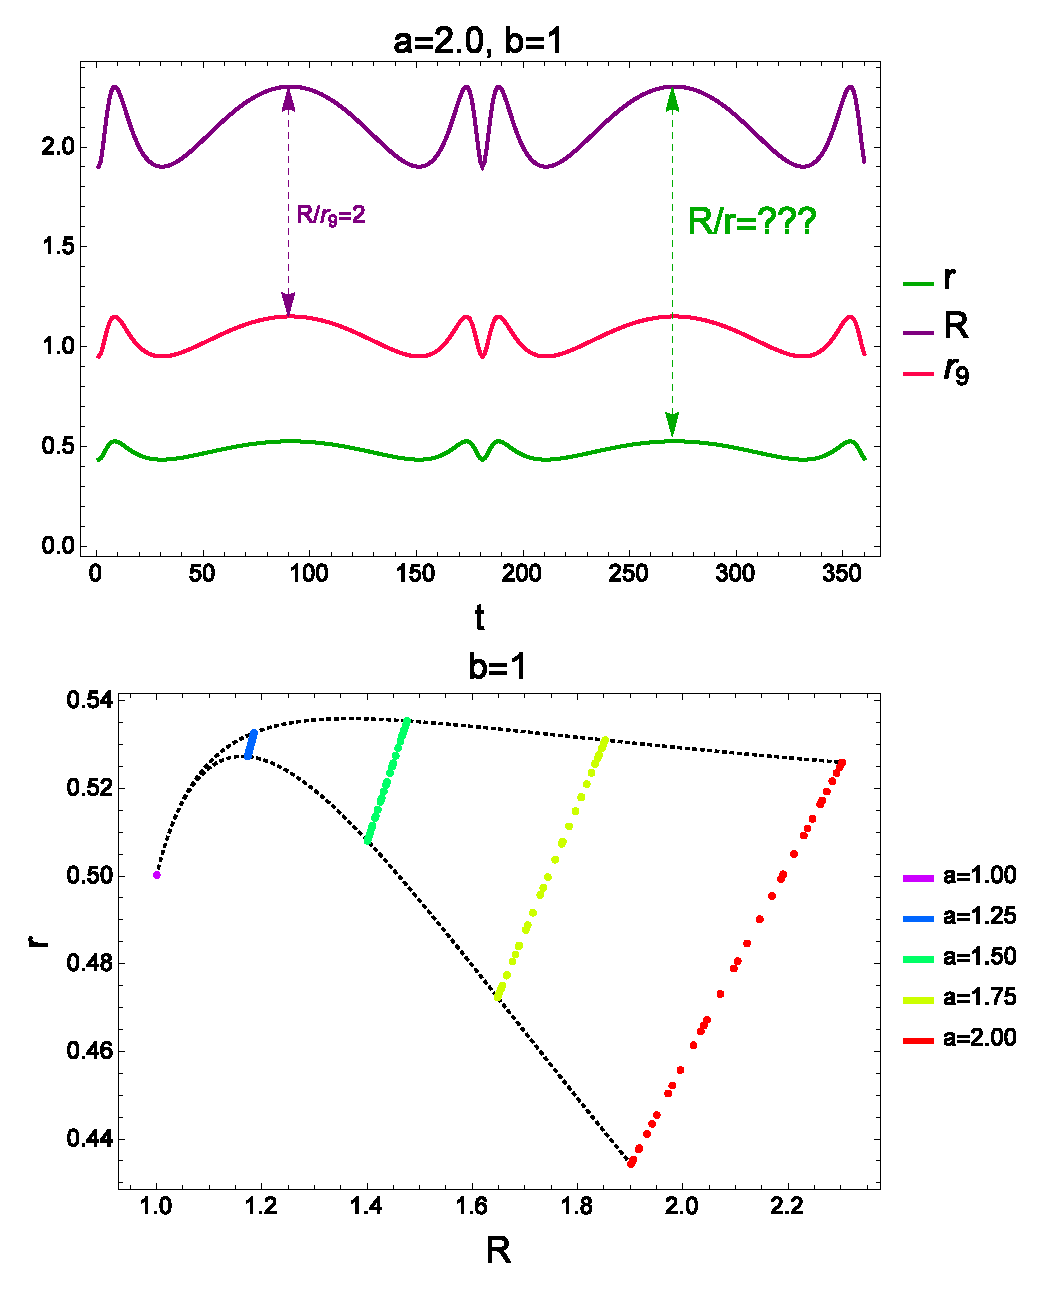
\includegraphics[width=0.70\textwidth]{1050_radii_grid2.eps}
    \caption{\textbf{Top}: The three radii (inradius $r$, circumradius $R$ and radius of the 9-point circle $r_9$ plotted vs. $t$ of $P_1(t)=(a \cos t,\sin t)$. $R/r_9=2$ holds for any triangle, though $R/r$ is not constant in general. \textbf{Bottom}: Scatter plot in $(r,R)$-space: each dot is a 3-periodic orbit in a discrete set of $a/b$ families. Each family of triangles organizes along a straight line, suggesting the $r/R$ ratio is constant. The minimum and maximum $(r,R)$ that can occur in a family are bound by two continuous curves (dotted black); see \eqref{eqn:rmin-rmax}.}
    \label{fig:radii-grid2}
\end{figure}

For illustration, Figure~\ref{fig:rovR-vs-ab} shows the monotonically decreasing dependence of $r/R$ vs. $a/b$.

\begin{figure}[H]
    \centering
    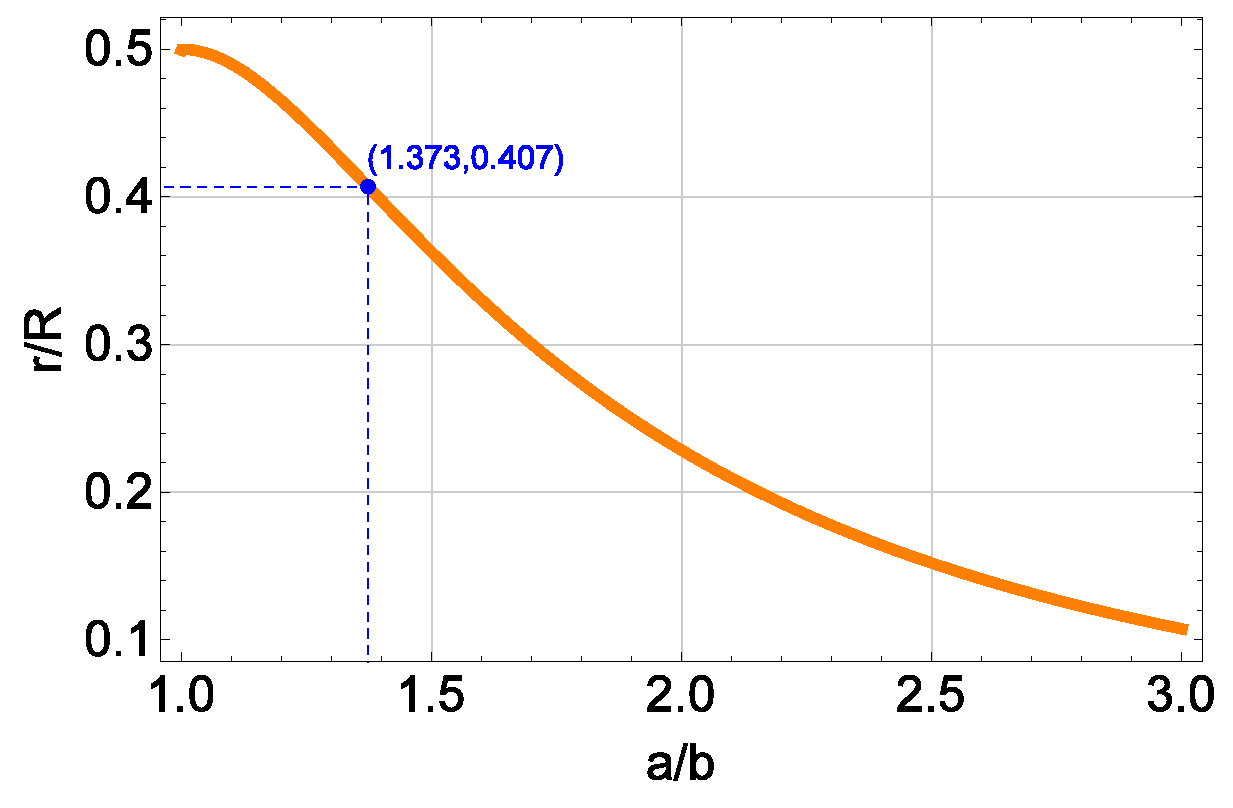
\includegraphics[width=.60\textwidth]{1030_rR_vs_ab.eps}
    \caption{Dependence of $r/R$ on the elliptic billiard aspect ratio $a/b$. The maximum is achieved when the elliptic billiard is a circle. The curve contains an inflection point that still lacks a geometric interpretation.}
    \label{fig:rovR-vs-ab}
\end{figure}


